%\documentclass[aip,pof,nofootinbib,reprint,onecolumn]{revtex4-1}
\documentclass[10pt,openany,onecolumn,a4wide,pof]{article}

\usepackage{amssymb,amsbsy,amsmath}
\usepackage[margin=1.0in]{geometry}
\usepackage[utf8]{inputenc}
\usepackage{xcolor}
\usepackage{graphicx,subfigure}
\usepackage[normalem]{ulem}
\usepackage{placeins}


%\input{tex_files/commandes}
%%%%%%%%%%%%%%%%%%%%%%%%%%%%%%%%%%%%%%%%%%%%%%
%%%%%%%%%%%%%%%%%%%%%%%%%%%%%%%%%%%%%%%%%%%%%%
%comments:
\newcommand{\mescom}[1]{{\color{red}{}#1}}
\newcommand{\issue}[1]{{\color{gray} #1 }}
\newcommand{\quest}[1]{{\color{blue} #1 }}
\newcommand{\todo}[1]{{\color{red} #1 }}


% shortcut
\newcommand{\gras}[1]{\boldsymbol{#1}}
\newcommand{\mypar}[1]{\left(#1\right)}
\newcommand{\mya}[1]{\left\{#1\right\}}
\newcommand{\norme}[1]{\left\Vert #1\right\Vert_2}




%%%%%%%%%% spaces
\newcommand{\Ephaz}{\mathcal{D}}%espace des phases
\newcommand{\Eobs}{\Omega}%espace des observables

%%%%%%%%%% dimensions
\newcommand{\Nphaz}{n_{\mathcal{D}}} % dim phases space
\newcommand{\Nm}{n_p} % dim obs space
\newcommand{\Nsnap}{N} % number of snapshots
\newcommand{\Ns}{n_s} % spatial discretisation number
\newcommand{\Np}{m}

%%%%%%%%%% functions
\newcommand{\fdyn}{f} % dyn function
\newcommand{\flot}{\mathfrak{f}} % flow operator
\newcommand{\costf}{J} % costfcuntion
\newcommand{\costff}{j} % under the int cost function
\newcommand{\lag}{\mathcal{L}} % Lagrangian function
\newcommand{\fint}{\mathfrak{F}} % 

%%%%%%%%%% variables
\newcommand{\obs}{y} % observable
\newcommand{\point}{\gras{x}} % point in space phase
\newcommand{\res}{\gras{\xi}} % a residu
\newcommand{\rpoint}{X}
\newcommand{\error}{\epsilon} % an error


%\input{tex_files/commandes_locales}

\begin{document}


%\input{tex_files/first_page}

\title{Note on implicit filters}

\author{Florimond Guéniat, Lionel Mathelin, Yussuf M. Hussaini}
%%\homepage{http://www.gueniat.fr}
%%\email{florimond.gueniat@limsi.fr}
%\author{Florimond Gu\'eniat}
%\affiliation{Department of mathematics, Florida State Univ., 32306-4510 Tallahassee, Fl, US}
%\author{Lionel Mathelin}
%\affiliation{LIMSI-CNRS, 91403 Orsay cedex, France}
%%\author{Omid Khanmohamadi}
%%\affiliation{Department of mathematics, Florida State Univ., 32306-4510 Tallahassee, Fl, US}
%\author{Yussuf Hussaini}
%\affiliation{Department of mathematics, Florida State Univ., 32306-4510 Tallahassee, Fl, US}
%
%
%
%\date{\today}
%
%
%
%\keywords{Data assimilation, Model identification}
%
%\begin{abstract}
%
%
%\end{abstract}

%\keywords{Dynamic Mode Decomposition, Compressed Sensing, Shannon-Nyquist criterion, large dataset, K-means}

\maketitle



%\input{tex_files/intro}
\section{Introduction}
\label{sec-intro}

In this article, the numerical cost and the accuracy of Implicit Particle Filter (IPF) are quantified, using Burgers's equation and shallow water equations as scenarios.
Identifying the uncertities in a data assimilation problem is specifically addressed.

IPF aims at estimating or the state, or the initial conditions or or some parameters of a system, by coupling a model and observations. 
A noise component can be present in both the observations and the model. 
Such an aim is of importance in many domains, most notably meteorology\todo{ref}, where initial conditions compatible with observations leads to accurate predictions. 
If not the case, as expected from a chaotic system, the accuracy of the forecast can drop significantly.
Seismography{ref} is an other field of importance for data assimilation, \emph{e.g.}, to locate epicenter.
It has been also successfully applied to nuclear fusion\footnote{Cacuci, D. G., \& Ionescu-Bujor, M. (2010). Best-Estimate model calibration and prediction through experimental data assimilation-I: Mathematical framework. Nuclear science and engineering, 165(1), 18-44.} and agronomy \footnote{Guerif, M., \& Duke, C. L. (2000). Adjustment procedures of a crop model to the site specific characteristics of soil and crop using remote sensing data assimilation. Agriculture, ecosystems \& environment, 81(1), 57-69.}.

When the model is linear, and the noise Gaussian, the most suited class of methods are the Kalman filters. 
Uncertaintities are directly related to the parameters of the Gaussian, which are totally determined by the Kalman filter. 
The generalization of Kalman filters, ensemble Kalman filters,~\cite{Evensen2009}, can deal with non-linear model by using replica (particles) of the system, to represent the prior density of solutions. 
Nevertheless, it performs poorly when the errors and noises are not Gaussian, \cite{Miller1999}. 
4D-Var and cost function-minimization techniques are very popular methods, giving usually accurate results, but they fail at quantifying the uncertainties in the results, with respect to the noise in the model and observations. 
The sensitivity analysis cannot be considered as accurate, as soon as the noise cannot be considered as small~\todo{cite Plessix, review}.
Moreover, results are actually biased if the posterior pdf is multimodal, \cite{Rabier1992}.

Indeed, IPF have been successfully used for data assimilation, \cite{Chorin2010}, system identification, \cite{Morzfeld2012}, and parameter estimation. 
It is particularly relevant for multimodal pdf ; it provides an unbiased estimate of the solutions, \cite{Atkins2013}.
As for Markov-Chain Monte Carlo method, IPF relies on a set of particles for the quantification of the conditional pdf of the system.
The main difference lies in the fact that only a few, weighted hence carefully chosen particles are considered.  
Identifying these particles is done through the maximisation of a tailor-constructed probability.
It ensures that each particle is associated with relevant informations of the pdf. 
The moments of the estimated pdf, as in standard MCMC methods, might be used for quantifying the uncertainties.

In this article, the precision and accuracy of IPF are qualitatively shown
and a roadmap for tackling the computational costs issue is proposed.

%\input{tex_files/DA}%
\section{4D-VAR}
\subsection{Preliminaries}
Let's consider the state vector $\point$ of a system of interest, evolving on the $\Nphaz$ manifold $\Ephaz $. This field is modelized through the set of equations $\fdyn$:

\begin{equation}
\fdyn(\point,\dot{\point},q,t) =0.
\label{eq-system}
\end{equation} 

The model might not be perfect. Flaws can come, for instance, from
uncertainties in the model parameters $q$ or in some initial conditions.
Consequently, a functional $\costf$ is introduced, in order to fit the model
by taking in account observations at hand:
\begin{equation}
\costf(\point,q) = \int_0^T  \costff(\point,q,t) dt.
\label{eq-def_cost}
\end{equation} 
For instance, one may want to minimize the discrepancy between the model predictions and some observations $\obs$:
$$\costff(\point,q,t) = \left|h(\point,q,t) - \obs(t)\right|^2$$ 

In the data assimilation context, the initial conditions are actually derived from the array of parameters $q\in\mathbb{R}^{n_q}$, with a relation $g:\Ephaz\times\mathbb{R}^{n_q}\rightarrow\mathbb{R}$:
$$g(\point(0),q) = 0.$$

Minimizing $\costf$ gives the best initial conditions, in the sense that Eq.~\eqref{eq-system} will produce fields as compatible as possible with the observations.

Efficient and reliable minimization methods, such as the BFGS\todo{ref}
method, need the gradient of the functional with respect to the parameters.
When $\Nphaz$ is large, approximating the gradient with finite differences
becomes impractical. A powerful alternative to computing the gradient is to
solve the adjoint equation\todo{ref}.
\subsection{Computing the gradient of the cost functional}

Identifying the minimum of the $\costf$ relies on the gradient of the
functional with respect to the parameters:
$D_q\costf = \frac{D\,\costf}{Dq}$. For that, one can introduce the
Lagrangian $\lag$, associated with the two Lagrange parameters $\lambda$ and
$\mu$:
\begin{equation}
  \lag\mypar{\point,\dot{\point},q,\lambda,\mu}
  =
  \int_0^T
  \bigg[
  \costff(\point,q,t) + \lambda^{\dagger}\fdyn(\point,\dot{\point},q,t)
  \bigg] dt + \mu^{\dagger} g(\point(0),q) 
\label{eq-lag}
\end{equation}
where $^{\dagger}$ is the transpose operator. Naturally, both $\point$ and $\dot{\point}$ are considered as variables.
As $\fdyn$ and $g$ are null by construction, $\lambda$ and $\mu$ can be designed specifically to alleviate the computations.
computations.
The gradient $D_q\lag = \frac{D\lag}{Dq}$ of $\lag$ is
\begin{equation}
\begin{split}
&D_q\lag\mypar{\point,\dot{\point},q,\lambda,\mu} = \int_0^T  \bigg[\partial_{\point}\costff(\point,q,t)d_q \point  +\partial_{q} \costff(\point,q,t) + \\
& \qquad \lambda^{\dagger} \partial_{\point}  \fdyn(\point,\dot{\point},q,t) d_q \point + \lambda^{\dagger}\partial_{\dot{\point}} \fdyn(\point,\dot{\point},q,t)d_q \dot{\point}  + \lambda^{\dagger}\partial_q\fdyn(\point,\dot{\point},q,t) \bigg]dt + \\
& \qquad \mu^{\dagger} \partial_{\point(0)} g(\point(0),q) dq_{\point(0)}  + \mu^{\dagger} \partial_q g(\point(0),q) .
\end{split}
\label{eq-deriv_lag}
\end{equation}
As a matter of facts, $D_q\lag = D_q \costf$.

The term in $d_{\dot{\point}}$ cannot be easily estimated. An integration by parts gives:

\begin{equation*}
\begin{split}
&\int_0^T\lambda^{\dagger}\partial_{\dot{\point}} \fdyn(\point,\dot{\point},q,t)d_q \dot{\point} dt = \\
&\qquad [\lambda^{\dagger}\partial_{\dot{\point}} \fdyn(\point,\dot{\point},q,t) d_q \point ]_0^T - \int_0^T \mya{\dot{\lambda}^{\dagger}\partial_{\dot{\point}} \fdyn(\point,\dot{\point},q,t) + \lambda^{\dagger}d_t\partial_{\dot{\point}}\fdyn(\point,\dot{\point},q,t)}d_q \point dt
\end{split}
\end{equation*}
The term associated with $d_{\dot{\point}}$ can now be replaced in Eq.~\eqref{eq-deriv_lag}.
Ordering terms in this equation leads to:

\begin{equation}
\begin{split}
&D_q\lag\mypar{\point,\dot{\point},q,\lambda,\mu} = \\
& \qquad \int_0^T  \bigg[  \mypar{\partial_{\point}\costff(\point,q,t) + \lambda^{\dagger} \partial_{\point}  \fdyn(\point,\dot{\point},q,t) - \mya{\dot{\lambda}^{\dagger}\partial_{\dot{\point}} \fdyn(\point,\dot{\point},q,t) + \lambda^{\dagger}d_t\partial_{\dot{\point}}\fdyn(\point,\dot{\point},q,t)}} d_q \point   +\\
& \qquad \partial_{q} \costff(\point,q,t)    + \lambda^{\dagger}\partial_q\fdyn(\point,\dot{\point},q,t) \bigg] dt + \\
& \qquad \mya{\mu^{\dagger} \partial_{\point} g(\point,q) - \lambda^{\dagger}\partial_{\dot{\point}} \fdyn(\point,\dot{\point},q,t) }|_0 dq_{\point(0)}  + \mu^{\dagger} \partial_q g(\point(0),q) + \mya{\lambda^{\dagger}\partial_{\dot{\point}} \fdyn(\point,\dot{\point},q,t)}|_T d_q \point(T)
\end{split}
\label{eq-deriv_ord}
\end{equation}

Proper choices for $\lambda$ and $\mu$ allow to simplify the expression of $D_q\lag$.
The choice of $\lambda\mypar{T} = 0$ actually nullifies the term $\mya{\lambda^{\dagger}\partial_{\dot{\point}} \fdyn(\point,\dot{\point},q,t)}|_T d_q \point(T)$.
Then, $\lambda$ can be chosen as the solution of the so-called adjoint equation:
$$
\mypar{\partial_{\point}\costff(\point,q,t) + \lambda^{\dagger} \partial_{\point}  \fdyn(\point,\dot{\point},q,t) - \mya{\dot{\lambda}^{\dagger}\partial_{\dot{\point}} \fdyn(\point,\dot{\point},q,t) + \lambda^{\dagger}d_t\partial_{\dot{\point}}\fdyn(\point,\dot{\point},q,t)}} = 0 
$$
integrated in backward time. 
Finally, the Lagrange parameter $\mu$ is set so it nullifies the component associated with $dq_{\point(0)}$:
$$ \mya{\mu^{\dagger} \partial_{\point} g(\point,q) - \lambda^{\dagger}\partial_{\dot{\point}} \fdyn(\point,\dot{\point},q,t) }|_0 = 0.$$
Then, computing $D_q\lag$, hence $ D_q\costf$, is achieved by the integration of:
\begin{equation}
D_q\costf\mypar{\point,q} = \int_0^T  \bigg[  \partial_{q} \costff(\point,q,t)    + \lambda^{\dagger}\partial_q\fdyn(\point,\dot{\point},q,t) \bigg] dt +   \mu^{\dagger} \partial_q g(\point(0),q).
\label{eq-J_adj}
\end{equation}




%\input{tex_files/system}
\section{System}
\label{sec-sys}

\subsection{Burgers' equation}
\label{ssec-burgers}
The Burgers' equation \todo{stochastic part ?}is:
$$ \partial_t \point + \frac{1}{2} \partial_z \point^2 - \nu \partial^2_{zz}\point = 0. $$
$\point$ evolves on an $\Nphaz$-dimensional manifold $\Ephaz$. 
We consider that it has been spatially discretized. The field $\point$ can hence be modelized by $\hat{\point}$ through a set of ordinary differential equations $ \fdyn(\hat{\point},\dot{\hat{\point}},q,t) =0.$
$$ \dot{\hat{\point}} + L(\hat{\point},q,t) + NL(\hat{\point},q,t) = 0 \equiv \fdyn(\hat{\point},\dot{\hat{\point}},q,t), $$
where $q\in \mathbb{R}^{q}$ are the parameters of the model.
The solution is discretized with $n_x$ points linearly spaced: $\hat{\point}\in \mathcal{R}^{n_x}$, following an implicit scheme, in order to solve the time integration by Newton iterations. 
The advection part is approached by a backward difference scheme.
Acting as a regularization force, the viscosity actually makes this scheme stable, as no shock can occur in the considered working range. \todo{reformulate this sentence}.
The dissipation part is approached by a central difference scheme.
The $\hat{\,}$ symbol is dropped in the following for the sake of readability:
\begin{equation}
 \frac{\point^{n+1}_i - \point^{n}_i}{\Delta t} + \point^{n+1}_i \frac{\point^{n+1}_i - \point^{n+1}_{i-1}}{\Delta z} - \nu \frac{\point^{n+1}_{i+1} -2 \point^{n+1}_i + \point^{n+1}_{i-1}}{\Delta z ^2} = 0.
\label{eq-fdyn_burgers}
\end{equation}
More information about the partial derivatives needed for solving the adjoint equation can be found in Sec.~\ref{an-burgers}.
\begin{figure}[t]
\center
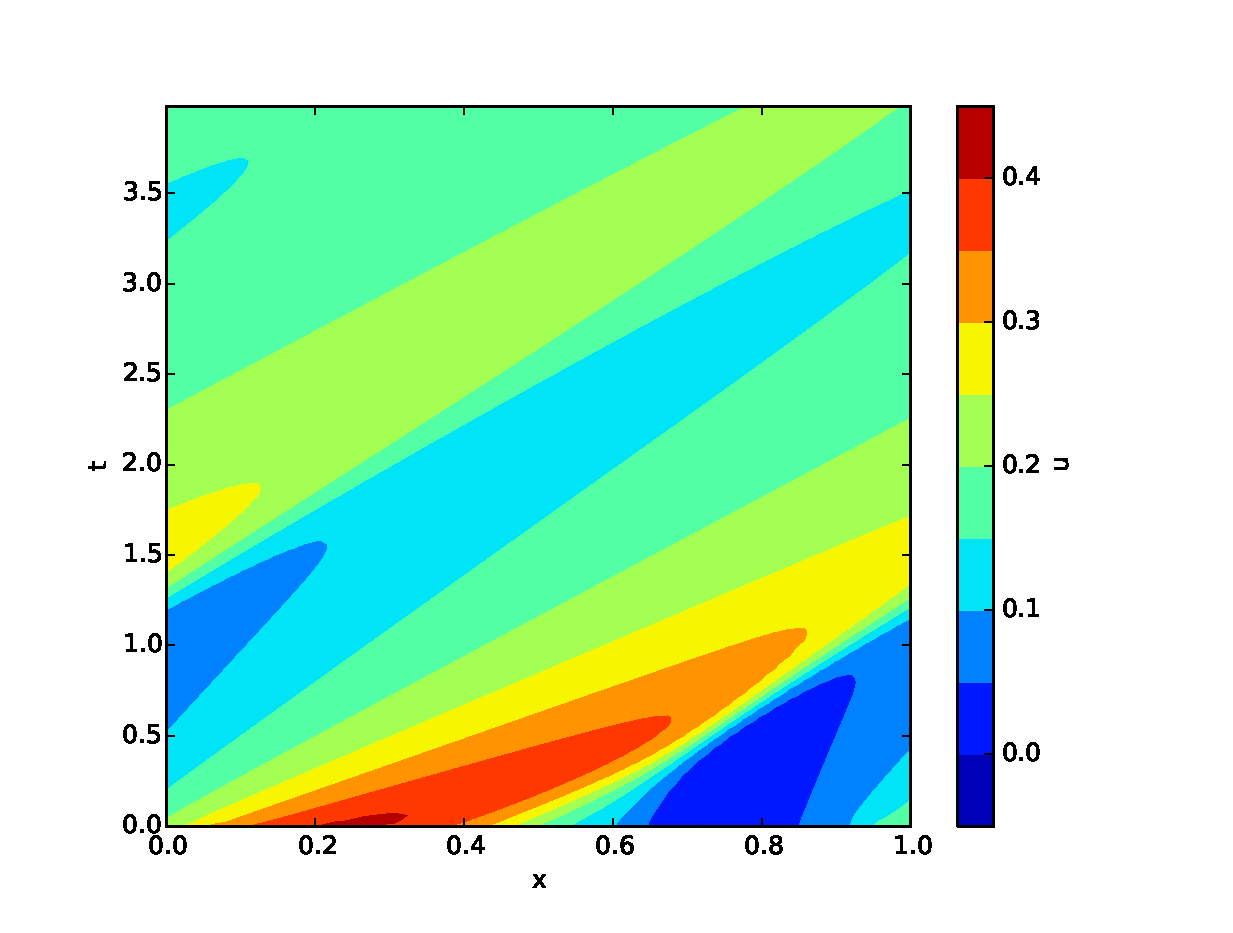
\includegraphics[height=.35\linewidth]{./burgers.eps}
\caption{\small Illustration of the Burgers' system.}
\label{fig-rmap}
\end{figure}


\subsection{Shallow water equations}  \label{ssec-swe}
\todo{We consider the \todo{SWE} equations (in its Ito form ?):
\begin{equation}
\begin{array}{lll}
\partial_t u & =& - u \partial_x u - v \partial_y u - f\,v - g \partial_x h -b\,u\\ 
\partial_t v & =& - u \partial_x v - v \partial_y v + f\,u - g \partial_y h -b\,v\\
\partial_t h & =& - \partial_x \mypar{\mypar{H+h}u} - \partial_y \mypar{\mypar{H+h}v}, \\
\end{array}
\label{eq-swe}
\end{equation} 
\todo{Ito ?} 0where $u$ and $v$ are the surface velocity, $h$ (resp. $H$) is the deviation of height (resp. mean height) from the botton. $f$ is the Coriolis coefficient and $\nu$ is the viscous drag coefficient. $g$ is the acceleration due to gravity.
This equation is spatially discretized.}

\begin{figure}[t]
\center
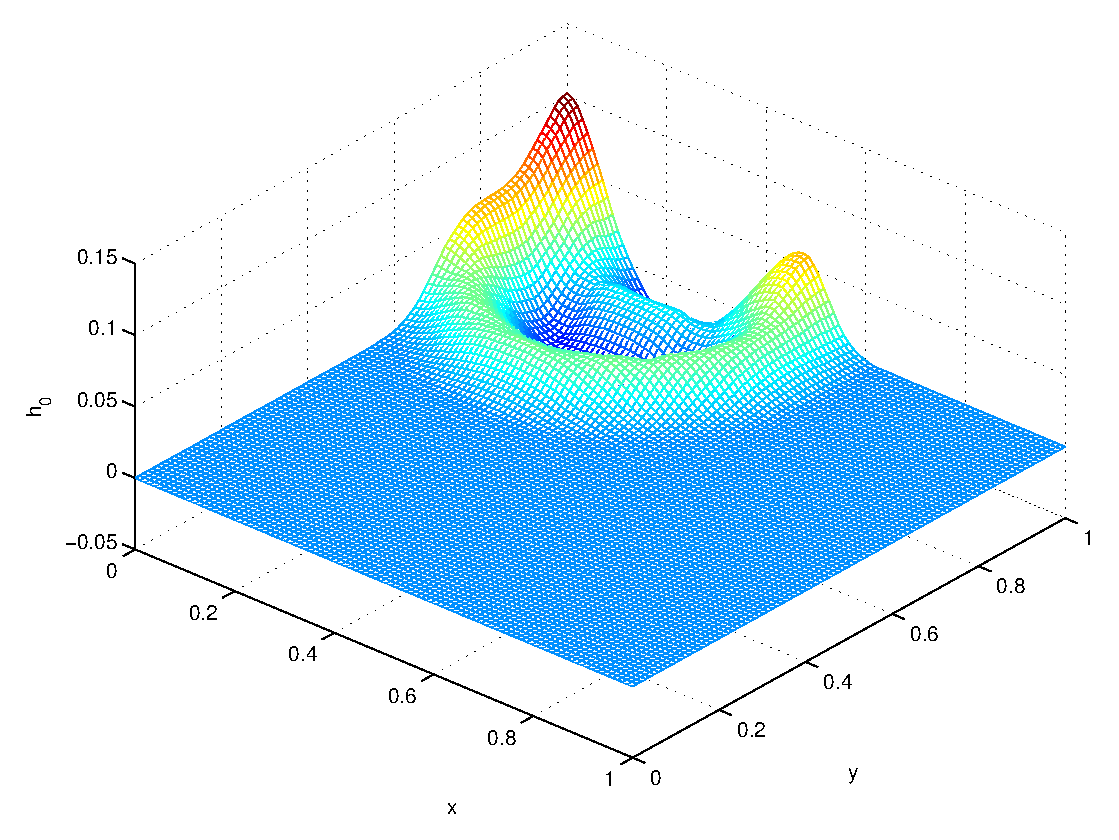
\includegraphics[height=.35\linewidth]{./SWE.eps}
\caption{\small Illustration of the initial conditions of the Shallow Water system.}
\label{fig-rmap}
\end{figure}


%\input{tex_files/IPF_algo}
\section{Particle methods and importance sampling}
\label{sec-ipf}
\subsection{Preliminaries}
Consider a stochastic dynamical system, in the Ito formalism, evolving on an $\Nphaz$-dimensional manifold $\Ephaz$:
\begin{equation}
d \point\mypar{t} = \flot\mypar{\point\mypar{t}}dt + \gras{G}dW, \qquad \point \in \Ephaz,
\label{eq-dyn}
\end{equation}
where $\point$ is the state of the system, $\flot:\Ephaz \rightarrow \Ephaz$
is the flow operator, $dW$ is a an $\Nphaz$-dimensional Brownian motion
(Wienner process), and $\gras{G}$ an $\Nphaz\times \Nphaz$ diffusion matrix.
With a proper time scheme\footnote{Kloeden, P. E., Platen, E. (1999).
  Numerical solution of stochastic differential equations. Berlin:
  Springer,\\ Klauder Petersen scheme} associated with a time step
$\delta t$, Eq.~\eqref{eq-dyn} becomes
\begin{equation}
\point\mypar{t_0+\mypar{n+1}\delta t} =  \fint\mypar{\point\mypar{t_0+n\delta t}}+\gras{G}\sqrt{\delta t} E,
\label{eq-TM}
\end{equation}
where $E$ is an $\Nphaz$-dimensional realization of the Wiener process. 
This model is to be understand as space and time discretization of a set of partial differential equations.

Let $h:\Ephaz \rightarrow \mathbb{R}^{\Nm}$ be a sensor function, so an observation on the system is:
\begin{equation}
 \obs(t) = h\mypar{x,t} + \sqrt{\gras{S}}Y,
\label{eq-obs}
\end{equation}
where $Y$ is an $\Nm$-dimensional, standard-normal random variable and
$\sqrt{\gras{S}}$ a covariance matrix. Let's also consider, without any loss
of generality, that $\gras{G} = g \gras{Id}$ and
$\sqrt{\gras{S}} = \sqrt{s} \gras{Id}$. In the following, the time will be
discretized accordingly to $\delta t$. For any variable $\star$,
$ \star\mypar{t_0+n\delta t}$ will be shortened as $ \star_n$.





\subsection{Probabilities derived from the Ito formulation}
The fact that noises in Eqs.~\eqref{eq-TM} and \eqref{eq-obs} are Gaussian does not mean that the probability density function (pdf) associated with the state of the system is Gaussian, as it will be shown in the following.


The probability that the $\Nphaz$-dimensional random variable $\rpoint^{n+1}$ coincide with a solution of the system described in Eq.~\eqref{eq-dyn}, at time $n+1$ and with the state $\point_{n}$ as initial condition, is given by
$$P^{\point_n,n+1}_{int}\mypar{\rpoint^{n+1}} = P\mypar{\rpoint^{n+1}|\point_n}.$$ 
This probability only depends on the system equations, \emph{i.e.} Eqs.~\eqref{eq-dyn} and \eqref{eq-TM}. When dealing with a Wiener process, the conditional probability is:
\begin{equation}
P^{\point_n,n+1}_{int}\mypar{\rpoint^{n+1}} \propto \exp \mypar{- \norme{\rpoint^{n+1} - \fint\mypar{\point_n}}^2/2\delta t g^2}.
\label{eq-proba_int}
\end{equation}
Note that if the noise is not Gaussian (\emph{i.e.} not described by a Wiener process), it only affects the right side of Eq.~\eqref{eq-proba_int}.

On an other hand, the probability that the observation of the variable $\rpoint^{n+1}$ is compatible with the observation of the system is given by
$$P^{n+1}_{obs}\mypar{\rpoint^{n+1}} = P\mypar{h\mypar{\rpoint^{n+1}}|\obs_{n+1}}.$$ 
Again, this probability only depends on the sensor function (see
Eq.~\eqref{eq-obs}):
\begin{equation}
 P^{n+1}_{obs}\mypar{\rpoint^{n+1}}  \propto \exp \mypar{- \norme{h\mypar{\rpoint^{n+1}} - y_{n+1}}^2/2s}.
\label{eq-proba_obs}
\end{equation}

From the Bayes' theorem, by combining Eq.~\eqref{eq-proba_int} and Eq.~\eqref{eq-proba_obs}, the probability $P^{\point_n,n+1}_{SI}$ that $\rpoint^{n+1}$ is a possible outcome from the previous state $\point_n$, given the observation $\obs_{n+1}$, is
\begin{equation}
P^{\point_n,n+1}_{SI}\mypar{\rpoint^{n+1}} \propto P^{\point_n,n+1}_{int}\mypar{\rpoint^{n+1}} P^{n+1}_{obs}\mypar{\rpoint^{n+1}}
\label{eq-bayes}
\end{equation}
From this writing, as a product, the pdf of $P^{\point_n,n+1}_{SI}$ is not normal.

Generalization is straightforward. 
Having several observations $\mya{\obs_{n+i}}_{\mya{i\in \mya{1,\hdots,r}}}$ available at hand, between time $t_n$ and $t_{n+r}$, is common. 
Consequently,  Eq.~\eqref{eq-bayes} becomes
\begin{equation}
P^{\point_n,n+r}_{SI}\mypar{\gras{\rpoint}_{n+1}^{n+r}} \propto \prod_{i=1}^r P^{\rpoint^{n+i-1},n+i}_{int}\mypar{\rpoint^{n+i}} \prod_{i\in \mya{1,\hdots,r}} P^{n_i}_{obs}\mypar{\rpoint^{n+i}},
\label{eq-SI}
\end{equation}
where $\gras{\rpoint}_{n+1}^{n+r} = \mya{\rpoint^{n+1}, \hdots,\rpoint^{n+r}}$ is now a $r\times\Nphaz$-dimensional random variable, coinciding with a potential trajectory of the state between $n+1$ and ${n+r}$. and with $\rpoint^n = \point_n$.

The probability $P^{n}_{DA}$ that the system is in a given state $\rpoint^n$ at the given time $n$ can be derived from Eq.~\eqref{eq-SI}:
\begin{equation}
P^{n}_{DA}\mypar{\gras{\rpoint}_{n}^{n+r}} \propto \prod_{i=1}^r P^{\rpoint^{n+i-1},n+i}_{int}\mypar{\rpoint^{n+i}} \prod_{i\in \mya{1,\hdots,r}} P^{n_i}_{obs}\mypar{\rpoint^{n+i}},
\label{eq-DA}
\end{equation}
with $\gras{\rpoint}_{n+1}^{n+r} = \mya{\rpoint^{n}, \hdots,\rpoint^{n+r}}$.

Data assimilation, as system identification, aims at identifying the state of the considered system, at any desired time. 
Consequently, $\chi \equiv \text{argmax}\mypar{P^{n}_{DA}}$ (resp. $\chi \equiv \text{argmax}P^{\point_n,n+r}_{SI}$) corresponds to the best solution of the data assimilation (resp. system identification) problem,~\cite{Chorin2010,Morzfeld2012,Atkins2013}. 
The form of Eqs.~\eqref{eq-proba_int} and \eqref{eq-proba_obs} implies that minimizing $F_{SI} = -\log P^{\point_n,n+r}_{SI}$ and $F_{DA} = -\log P^{n}_{DA}$ is numerically preferable.


In the following, the notation $P$ (resp. $F$) will refer indistinctly to $P^{\point_n,n+r}_{SI}$ or $P^{n}_{DA}$ (resp. $F_{SI}$ or $F_{DA}$), when no confusion is possible. 
Similarly, $X$ will refer to the considered random variable, and its dimension will be short-named $\Nphaz$.

Identifying the maximum can be, alternatively, efficiently done by 4D-VAR, \todo{refs}, when the distribution associated with $P_{DA}$ is known to be mono-modal\footnote{if note, the estimation might be biased. Weir 2013}.

For state identification, as for data assimilation, the initial conditions $\point_n$ in Eq.~\eqref{eq-SI} are often unknown. 
This problem is usually tackled by considering $\Np$ particles, \emph{i.e.} replicas of the system\footnote{\emph{e.g.}, in Markov Chain Monte Carlo simulations}.
For each particle $i$, an initial condition $\point_n^i$ is guessed. 
Maxima are computed from Eq.~\eqref{eq-SI}, for all the initial guesses. 

By the law of large numbers, it allows to estimate the moments of the pdf, that is, for system identification, the mean state $\point_n$, by averaging the results. 


Estimating the moments of the a given pdf might need a consequent number of particles\todo{refs}, and both the storage and the identification of samples from that pdf might be near to impossible.
Actually, when strictly following the law of large numbers, all the particles has the same importance.
An option is, instead of drawing random particles, to identify particles more representative of the probability density function (pdf) associated with $P$. 
Hence, less particles are needed for an accurate estimation of the pdf properties.

\subsection{Importance sampling}

Intuitively, a particle carries more information on the probability, as soon as it is associated with a high probability in Eq.~\eqref{eq-bayes} (resp. \eqref{eq-SI} or \eqref{eq-DA}).
Moreover, estimations of the pdf properties rely on drawing samples from the pdf. 
A sample has to be a possible outcome of the physical system described by Eq.~\eqref{eq-dyn} for being meaningful.

Importance sampling, \cite{Chorin2010,Morzfeld2012}, \todo{ref is} allows to tackle both these issues.
The key is to consider an easy-to-sample pdf $p$. Some samples $\rpoint_i$ are drawn from it. These samples are mapped with the the actually hard-to-sample pdf $P$.
It also provides a quantification of the importance of each sample with respect to the pdf, namely the weight of each particle, so the estimation of the moments are not biased.

The weights of $\rpoint_i$ are
\begin{equation}
w\mypar{\rpoint_i} = \frac{P\mypar{\rpoint_i}}{p\mypar{\rpoint_i}}.
\label{eq-weight}
\end{equation}

For being efficient, it is necessary that the maxima of $p$ and $P$ coincide. If not, some particles will be associated with low weights, and are hence of a low importance. Because of potential storage limitations and computational costs, such particles are to be avoided, and the objective is to identify particles with comparable weights.


In order to construct a $p$ density, let consider $\xi$, an intermediate
random variable. $\xi$ is drawn from a $\Nphaz$-dimensional Gaussian pdf.
Such a variable is, of course, far from being a possible outcome of the
physical system. It will be used as an intermediate for identifying a high
probability sample $\rpoint$, solution of the algebraic equation,
\cite{Morzfeld2012}:

\begin{equation}
F\mypar{\rpoint} - \Phi_F = \xi^t\xi/2,
\label{eq-alg}
\end{equation}
where $\Phi_F = F\mypar{\chi}$ is the given minimum of $F$, identified for instance with a 4D-VAR method.

The sample $X$ has then an high probability to remains close to $\chi$, as $\xi$ is drawn for a $0$ mean pdf. 

In order to identify the weight from Eq.~\eqref{eq-weight}, one has to compute the probability $p_{\rpoint}\mypar{\rpoint}$ of drawing $X$ from Eq.~\eqref{eq-alg}.
By the substitution rule, $p_X$ is related to the probability $P_{\xi}\mypar{\xi}$ of drawing the sample $\xi$ by
$$
p_{\rpoint}\mypar{\rpoint} \left|\det \frac{\partial \rpoint}{\partial \xi}\right|  = P_{\xi}\mypar{\xi}.
$$
Consequently, with Eq.~\eqref{eq-weight}, the weight associated to the sample $\rpoint$ is
\begin{equation}
w\mypar{\rpoint} = \frac{P\mypar{\rpoint}}{P_{\xi}\mypar{\xi}/\left|\det \frac{\partial \rpoint}{\partial \xi}\right|}.
\label{eq-weight_dev}
\end{equation}




\subsection{Random map}
\begin{figure}[t]
\center
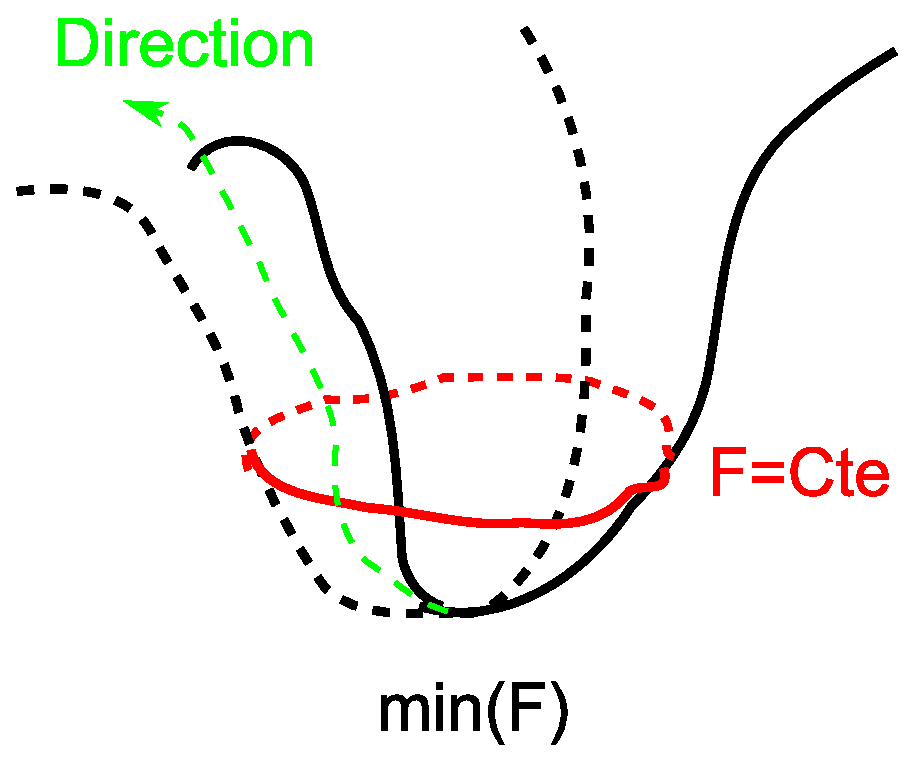
\includegraphics[height=.25\linewidth]{./min.eps}
\caption{\small Illustration of the methodology for drawing samples. The red curve corresponds to iso-values of $F\mypar{\rpoint} = Fmin+1/2 \xi^T\xi$. The green curve illustrate the random direction associated with $\xi$. The sample is found at the intersection of these two curves.}
\label{fig-rmap}
\end{figure}

Solving Eq.~\eqref{eq-alg} is a necessary step. For that, Morzfeld \emph{et al.}~\cite{Morzfeld2012} proposed to use the following ansatz:
\begin{equation}
\rpoint = \rpoint\mypar{\lambda} = \chi + \lambda L^t \xi/\sqrt{\xi^t \xi},
\label{eq-ansatz}
\end{equation}
where $\lambda$ is a real parameter, and $L^t$ is the Choleski decomposition of $H^{-1}$, $H$ being the Hessian of $F$, evaluated in $\chi$.
It minimizes the dispersion of the jacobian $\left|\det \frac{\partial \rpoint}{\partial \xi}\right|$ when considering different particles, and hence the dispersion of weights,~\cite{Morzfeld2012}.

A BFGS-algorithm is then used for identifying the $\lambda$ minimizing Eq.~\eqref{eq-alg}.

Computing the weight needs the evaluation of the jacobian of the maps between the reference sample $\rpoint$ and the random variable $\xi$.
Following~\cite{Morzfeld2012}, let be $\rho = \sqrt{\xi^t \xi}$.

Differentiating Eq.~\eqref{eq-ansatz} leads to

\begin{equation}
\begin{array}{lll}
\frac{\partial \rpoint}{\partial \xi} &=& \frac{\partial}{\partial \xi} \lambda L^t \xi/\sqrt{\xi^t \xi}\\
 &=& L^t \mypar{\frac{\partial\lambda}{\partial \xi} \xi/\sqrt{\xi^t \xi} + \lambda \frac{\partial}{\partial \xi} \xi/\sqrt{\xi^t \xi} }\\
\end{array}
\end{equation}



%\input{tex_files/results}
\section{Results}
\label{sec-results}

%\subsection{Dynamical systems}  \label{sec-results-Lorenz}
%To illustrate the methodology discussed above, we now consider the Lorenz' 63 system presented is Sec.~\ref{sec-sys}.
%The objective is the identification of the position of system, at each time (including initial conditions), knowing only some observations.
%
%The initial conditions, fixed to $\point_0 = \mypar{-4.4090617 ,   0.94099541,  31.65011104}$, are considered as not known. 
%The time step for the integration, using the Klauder-Perterson scheme, is $\delta t = 0.01$.
%
%The observable on the system is chosen to be unfavourable, with possible cancellation:
%\begin{equation}
%\gras{h}\mypar{\point,t} = \left|\sum z_i\right|
%\end{equation}
%
%
%In this example, the system is chaotic. It means that computing the future positions of the system is not possible without an \emph{exact} knowledge the previous positions. 
%Moreover, the system is stochastic ; computing the future positions of the system is not possible without an update knowledge of the influence of the noise.
%The sampling strategy is that an observable is at hand every five time steps, see Fig.~\ref{fig-lorobs}.
%
%One can see that the state phase is accurately followed, see specifically Fig.~\ref{sfig-lor_2dmean} and Figs.~\ref{fig-lor3d}. 
%
%
%
%\begin{figure*}[t]
%\center
%\includegraphics[height=.25\linewidth]{./fig/lorenz_obs.eps}
%\caption{\small Collected observables, in red.}
%\label{fig-lorobs}
%\end{figure*}
%
%\begin{figure*}[t]
%\center
%\subfigure[]{
%\includegraphics[height=.25\linewidth]{./fig/lorenz_full2D_zoom.eps}
%\label{sfig-lor_2dfull}
%}
%\hspace{3em}
%\subfigure[]{
%\includegraphics[height=.25\linewidth]{./fig/lorenz_mean2D.eps}
%\label{sfig-lor_2dmean}
%}
%\vspace{-1em}
%\caption{\small Identified Lorenz' system in black. Actual system solid red. $z_1$ component (a): all the particles (zoom). (b): mean of the particles. }
%\label{fig-lor2d}
%\end{figure*}
%
%\begin{figure*}[t]
%\center
%\subfigure[]{
%\includegraphics[height=.25\linewidth]{./fig/lorenz_full3D.eps}
%\label{sfig-lor_3dfull}
%}
%\hspace{3em}
%\subfigure[]{
%\includegraphics[height=.25\linewidth]{./fig/lorenz_mean3D.eps}
%\label{sfig-lor_3dmean}
%}
%\vspace{-1em}
%\caption{\small Identified Lorenz' system in black. Actual system solid red. (a): all the particles. (b): mean of the particles.}
%\label{fig-lor3d}
%\end{figure*}


%\input{tex_files/ideas}

\subsection{Burgers' equation}  \label{ssec-results-burgers}
To illustrate the methodology discussed above, we now consider the Burgers' equation presented is Sec.~\ref{ssec-burgers}.
The objective is the identification of the initial conditions, knowing only some observations. 
The accuracy and the computational costs are estimated. 
Three main parameters are allowed to variate: the noises in the model g, the noises in the observations s, and finally the dimensions (spatial ? temp?).

\begin{figure}[h]
\center
\subfigure[]{
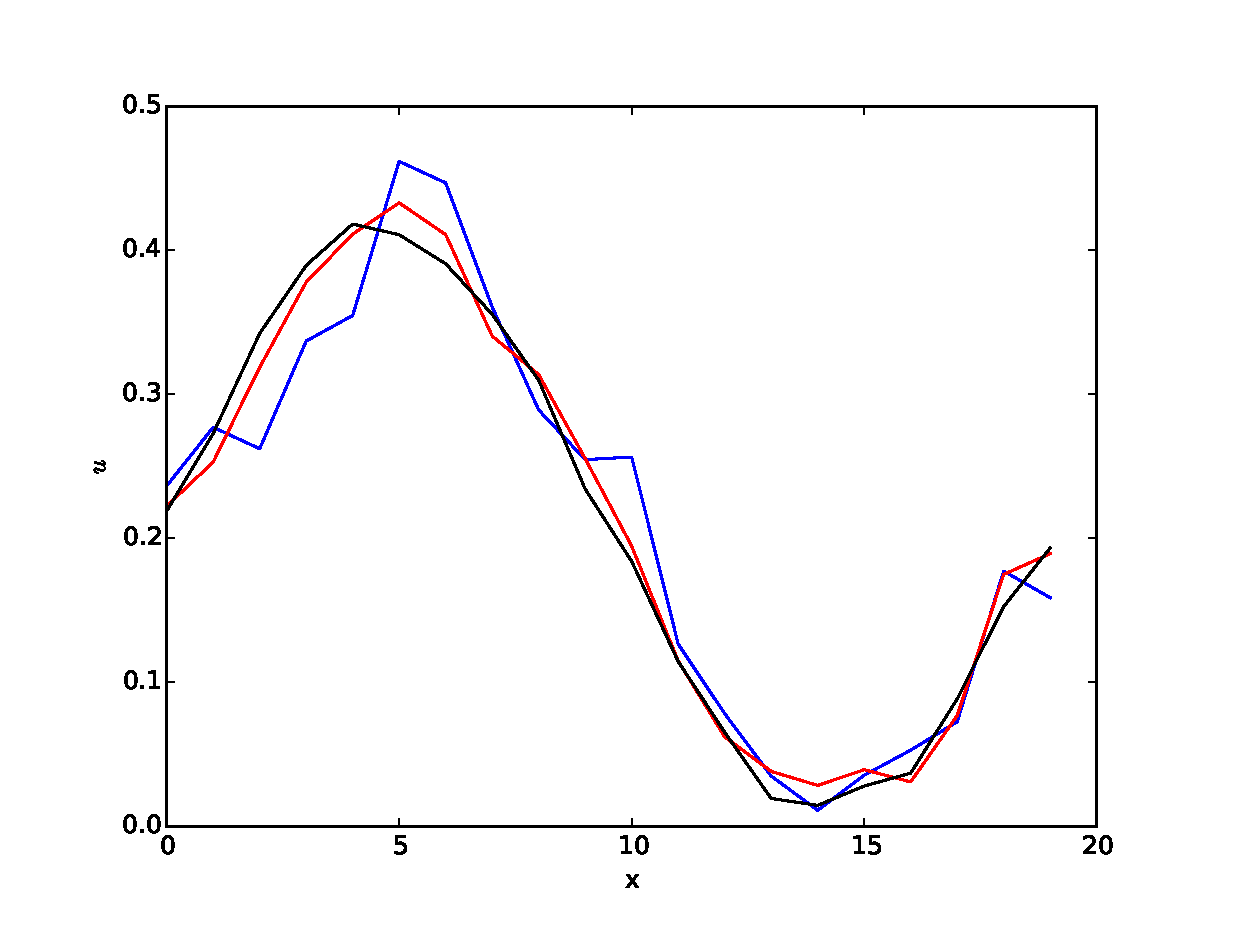
\includegraphics[width=.28\linewidth]{./burgers_local_comp.eps}
\label{sfig-trans}
}
\subfigure[]{
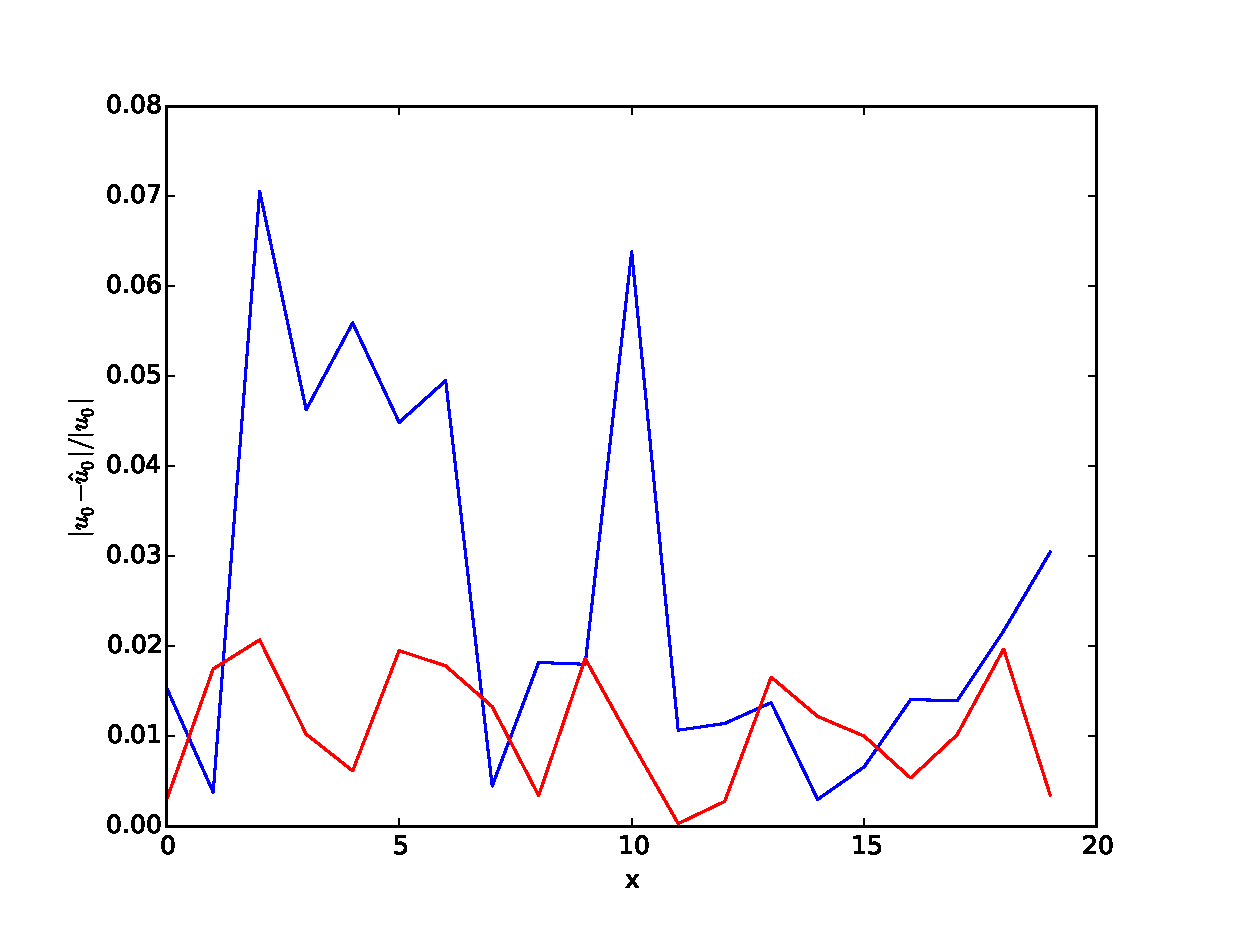
\includegraphics[width=.28\linewidth]{./burgers_local_comp_err.eps}
\label{sfig-rew}
}
\vspace{-1em}
\caption{\small (a): In black: Initial conditions. In red: approximation of the initial conditions with IPF. In Blue: approximation of the initial conditions with 4DVAR. (b): In red: errors to the initial conditions with IPF. In Blue: errors to the initial conditions with 4DVAR.}
\label{fig-err}
\end{figure}

\subsubsection{accuracy}

\begin{table}[h!]
\caption{
Comparison of mean errors $\error = \norme{\hat{\point}_0-\point_0}/\norme{\point_0}$, on $100$ runs, on the identification of the initial conditions $\point_0$, when $\hat{\point}_0$ is identified with 4D-Var and IPF. $\Ns=20$ spatial points were used for the spatial discretization, and $\Nsnap = 3$ snapshots are considered.
}
\begin{centering}
\begin{tabular}{c|ll|ll|ll}
$s$  & \multicolumn{2}{|c}{ $ 1.0\times 10^{-5} $ } & \multicolumn{2}{|c}{ $ 3.2\times 10^{-4} $ } & \multicolumn{2}{|c}{ $ 1.0\times 10^{-2} $ }  \\ 
\hline 
  & {\scriptsize 4D-Var} & {\scriptsize IPF} & {\scriptsize 4D-Var} & {\scriptsize IPF} & {\scriptsize 4D-Var} & {\scriptsize IPF} \\ 
\hline 
$ g=      1.0\times 10^{-5}$ & $7.6\times 10^{-3}$ & $3.2\times 10^{-5}$ & $7.6\times 10^{-3}$ & $1.0\times 10^{-3}$ & $4.8\times 10^{-2}$ & $4.6\times 10^{-2}$ \\ 
$g=      3.2\times 10^{-4} $ & $7.6\times 10^{-3}$ & $4.0\times 10^{-5}$ & $7.7\times 10^{-3}$ & $1.7\times 10^{-3}$ & $4.7\times 10^{-2}$ & $3.1\times 10^{-2}$ \\ 
$ g=      1.0\times 10^{-2}$ & $ 2.1\times 10^{-2}$ & $5.9\times 10^{-6}$ & $?\times 10^{-?}$ & $?\times 10^{-?}$ & $?\times 10^{-?}$ & $?\times 10^{-?}$ \\ 
\end{tabular}
\label{tab-mean_errors_burgers}
\end{centering}
\end{table}

\begin{table}[h!]
\caption{
Comparison of deviation of errors $\error = \norme{\hat{\point}_0-\point_0}/\norme{\point_0}$, on $100$ runs, on the identification of the initial conditions $\point_0$, when $\hat{\point}_0$ is identified with 4D-Var and IPF. $\Ns=20$ spatial points were used for the spatial discretization, and $\Nsnap = 3$ snapshots are considered.
}
\begin{centering}
\begin{tabular}{c|ll|ll|ll}
$s$  & \multicolumn{2}{|c}{ $ 1.0\times 10^{-5} $ } & \multicolumn{2}{|c}{ $ 3.2\times 10^{-4} $ } & \multicolumn{2}{|c}{ $ 1.0\times 10^{-2} $ }  \\ 
\hline 
  & {\scriptsize 4D-Var} & {\scriptsize IPF} & {\scriptsize 4D-Var} & {\scriptsize IPF} & {\scriptsize 4D-Var} & {\scriptsize IPF} \\ 
\hline 
$ g=      1.0\times 10^{-5}$ & $8.6\times 10^{-4}$ & $5.5\times 10^{-6}$ & $9.0\times 10^{-4}$ & $1.6\times 10^{-4}$ & $7.7\times 10^{-3}$ & $7.1\times 10^{-3}$ \\ 
$g=      3.2\times 10^{-4} $ & $8.4\times 10^{-4}$ & $6.2\times 10^{-6}$ & $1.0\times 10^{-3}$ & $1.7\times 10^{-4}$ & $8.6\times 10^{-3}$ & $4.9\times 10^{-3}$ \\ 
$ g=      1.0\times 10^{-2}$ & $9.3\times 10^{-2}$ & $1.4\times 10^{-5}$ & $?\times 10^{-?}$ & $?\times 10^{-?}$ & $?\times 10^{-?}$ & $?\times 10^{-?}$ \\ 
\end{tabular}
\label{tab-std_errors_burgers}
\end{centering}
\end{table}


\begin{itemize}
\item noise in model
\item noise in observation
\item dimensions
\end{itemize}
\subsubsection{Computational costs}
\begin{itemize}
\item noise in model
\item noise in observation
\item dimensions
\end{itemize}



\section*{BIBLIOGRAPHY}
\bibliographystyle{ieeetr}
\bibliography{small_biblio}
\appendix
\section{Burgers' equation and adjoint equations}
\label{an-burgers}
We recall here the expression from Eq.~\eqref{eq-fdyn_burgers}:
$$ \frac{\point^{n+1}_i - \point^{n}_i}{\Delta t} + \point^{n+1}_i \frac{\point^{n+1}_i - \point^{n+1}_{i-1}}{\Delta z} - \nu \frac{\point^{n+1}_{i+1} -2 \point^{n+1}_i + \point^{n+1}_{i-1}}{\Delta z ^2} = 0 $$
The route "discretization then adjoint" is hence followed.

As a matter of fact, the $i$th component of $\fdyn$ is:
$$\fdyn_i\mypar{\point,\dot{\point},q,t} = \dot{\point_i} + \point_i \frac{\point_i - \point_{i-1}}{\Delta z} - \nu \frac{\point_{i+1} -2 \point_i + \point_{i-1}}{\Delta z ^2}. $$
Consequently, the partial derivatives with respect to $\point$ are
$$\partial_{\point_j} \fdyn_i\mypar{\point,\dot{\point},q,t} = \frac{1}{\Delta z }\mypar{2 \point_i \delta_{i,j} - \delta_{i-1,j}} + \frac{1}{\Delta z ^2}\mypar{\delta_{i+1,j} - 2 \delta_{i,j} + \delta_{i+1,j}}.$$
The partial derivative with respect to $\dot{\point}$ is
$$\partial_{\dot{\point}} \fdyn\mypar{\point,\dot{\point},q,t}  = Id,$$
and then $$dt\partial_{\dot{\point}} \fdyn\mypar{\point,\dot{\point},q,t}  = 0. $$

$$\partial_{\dot{\point}} \fdyn\mypar{\point,\dot{\point},q,t}  = Id,$$
and then $$dt\partial_{\dot{\point}} \fdyn\mypar{\point,\dot{\point},q,t}  = 0. $$

The cost function is associated with
$$\costff\mypar{\point,q,t} = || \point-\obs(t)||^2.$$
Hence, the partial derivatives with respect to $q$ and $\point$ are
$$\partial_q \costff\mypar{\point,q,t} = 0,$$
and
$$\partial_{\point} \costff\mypar{\point,q,t} = 2*\mypar{\point-\obs(t)}.$$

The parameters $q$ are actually the initial conditions. Hence, $n_q$ is equal to $\Nphaz$. As a matter of fact, $g$ is:
$$g(\point(0),q) = \point(0)-q = 0.$$
Then, the partial derivatives of $g$ follow:
$$\partial_q g(\point(0),q) = -Id,$$
and
$$\partial_u g(\point,q)|_0 = Id.$$

\end{document}